\section{Comparison}
\label{sect:results:comparison}
\subsection{Assumptions}
This comparison must be seen in the context of a number of assumptions
about the systems being compared. With regards to fairness, it is important to
note that the algebra trees generated by Pathfinder may have been
optimised (to which the exact extent is not known), while the algebra trees
generated by the prototype developed throughout this project \emph{does not apply any optimalisations} at all. The
optimalisations applied by Pathfinder are noted
in \cite{pathfinder_purelyRelational}.

Some important effects on the Pathfinder algebra tree from these
optimalisations are:
\begin{itemize}
  \item The cartesian products between a loop relation and a constant
  subexpression are transformed into projections
  \item The custom operator \textsf{attach} is roughly a simpler equivalent to
  the \textsf{make()} operator in MQL (see section \ref{sect:method:mql}, page
  \pageref{sect:method:mql})
\end{itemize}
TODO: noe mer her?

\newpage
\subsection{DAG comparison}
Note that the readability for these DAG comparisons are not essential --
however, links to large-scale versions of these diagrams are noted in appendix
\ref{appendix:links_and_resources}.

\begin{figure}[!h]
	\centering
	\mbox{
		\subfigure[Pathfinder/MonetDB]{		
			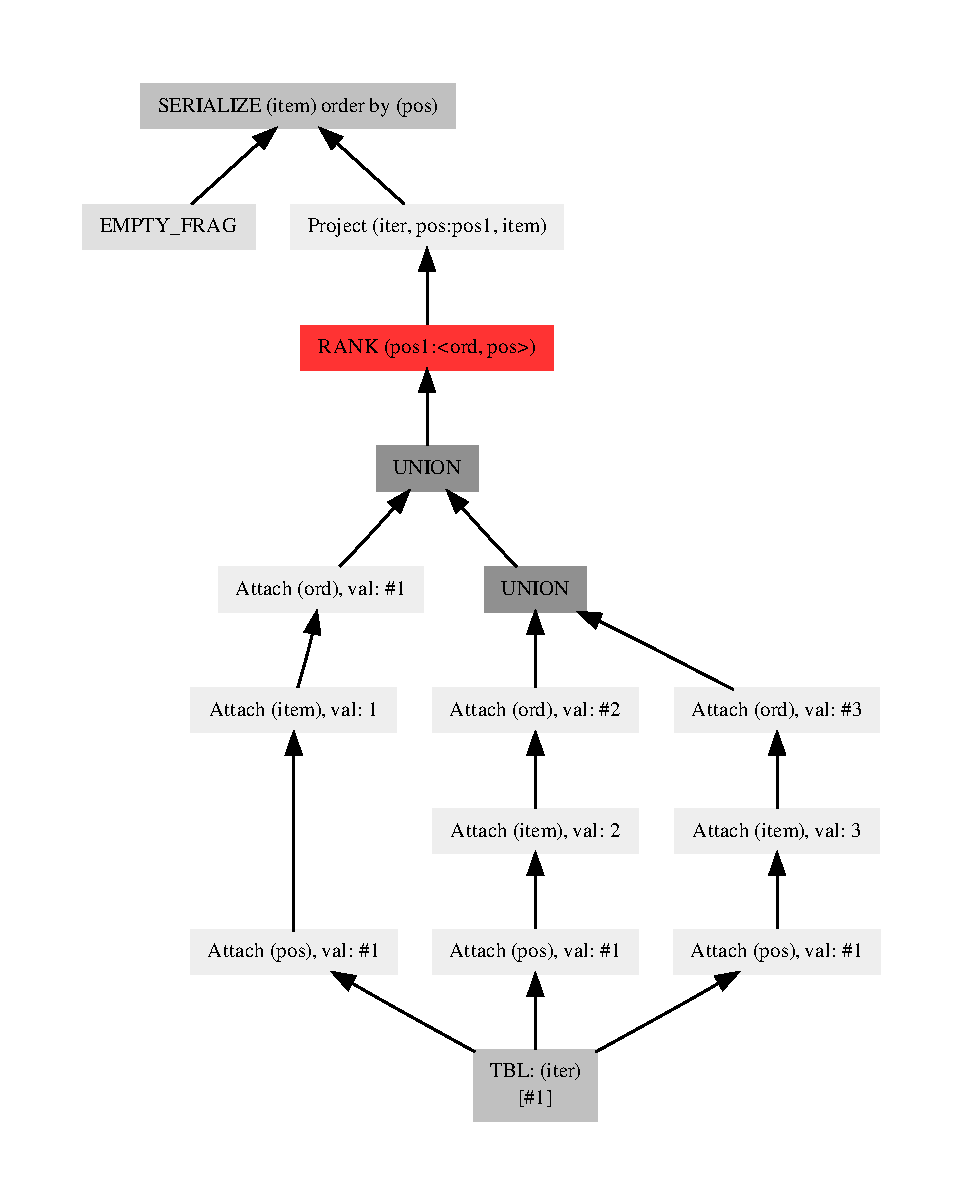
\includegraphics[width=0.4\textwidth]{img/graphs/td_impl_flwor_simple_pathfinder}
			\label{fig:result:comparison:simple_dag}
		}
		\quad
		\subfigure[Prototype implementation]{
		
			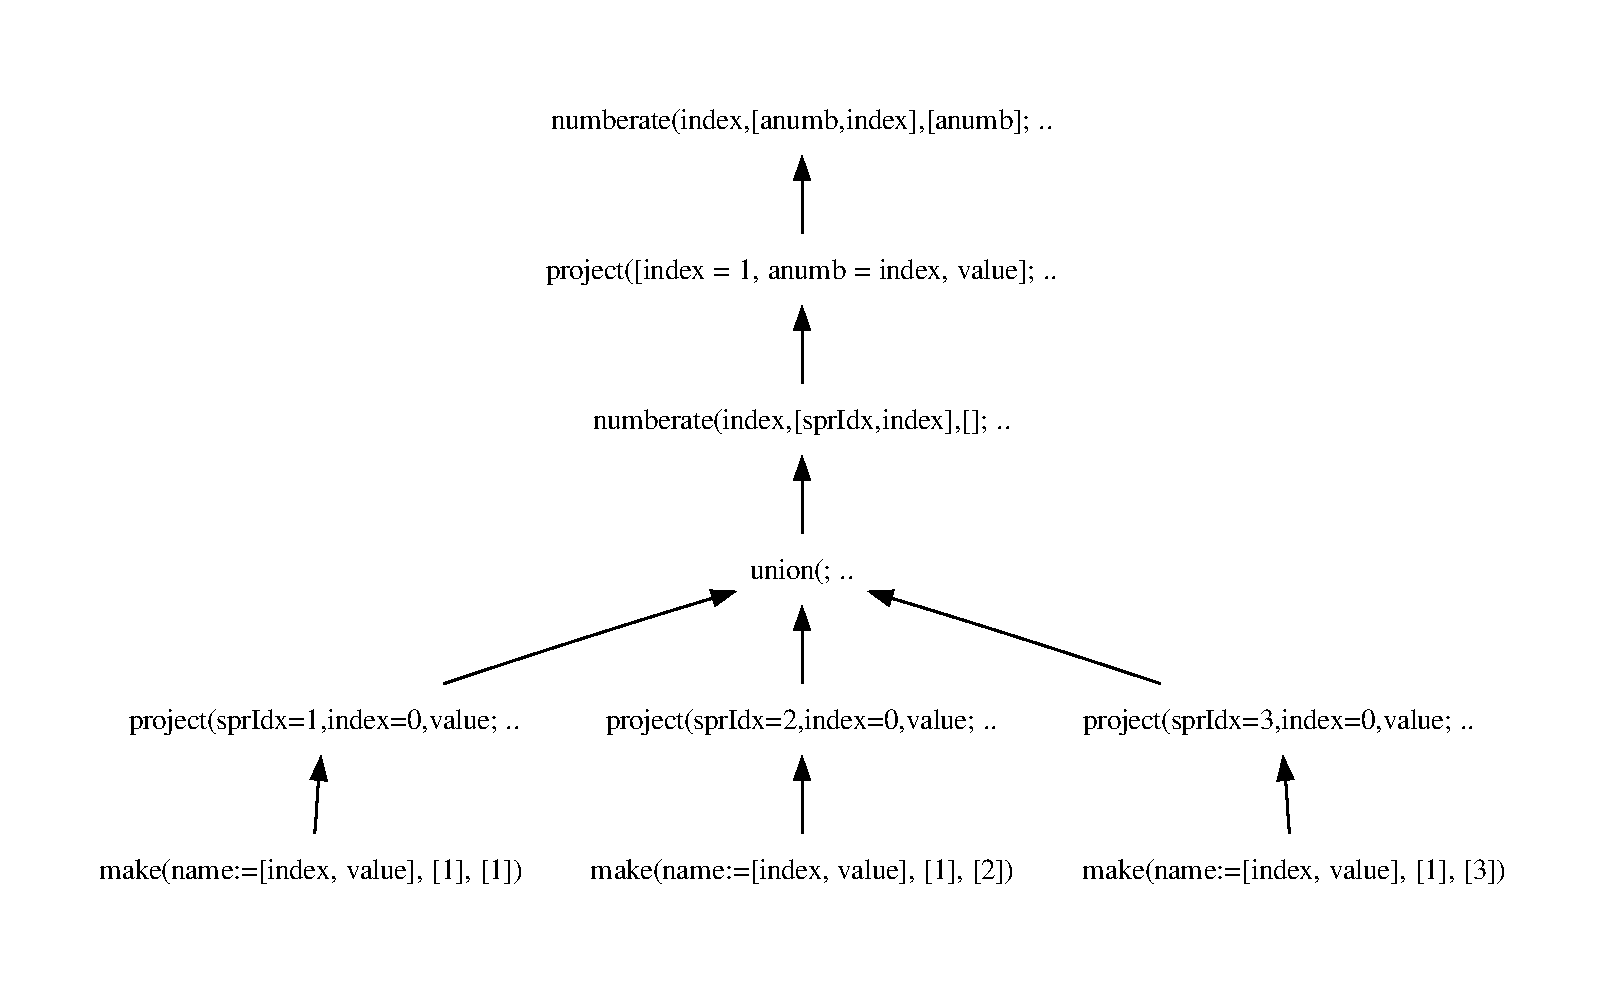
\includegraphics[width=0.6\textwidth]{img/graphs/td_impl_flwor_simple_xq_relalg}
			\label{fig:result:comparison:simple_pathfinder_dag}
		}
	}
	\caption{Comparison of DAGs for the trivial expression in section
	\ref{sect:results:algebra:generated:trivial_flwor}}
\end{figure}

\newpage
\begin{figure}[!h]
	\centering
	\mbox{
		\subfigure[Pathfinder/MonetDB]{		
			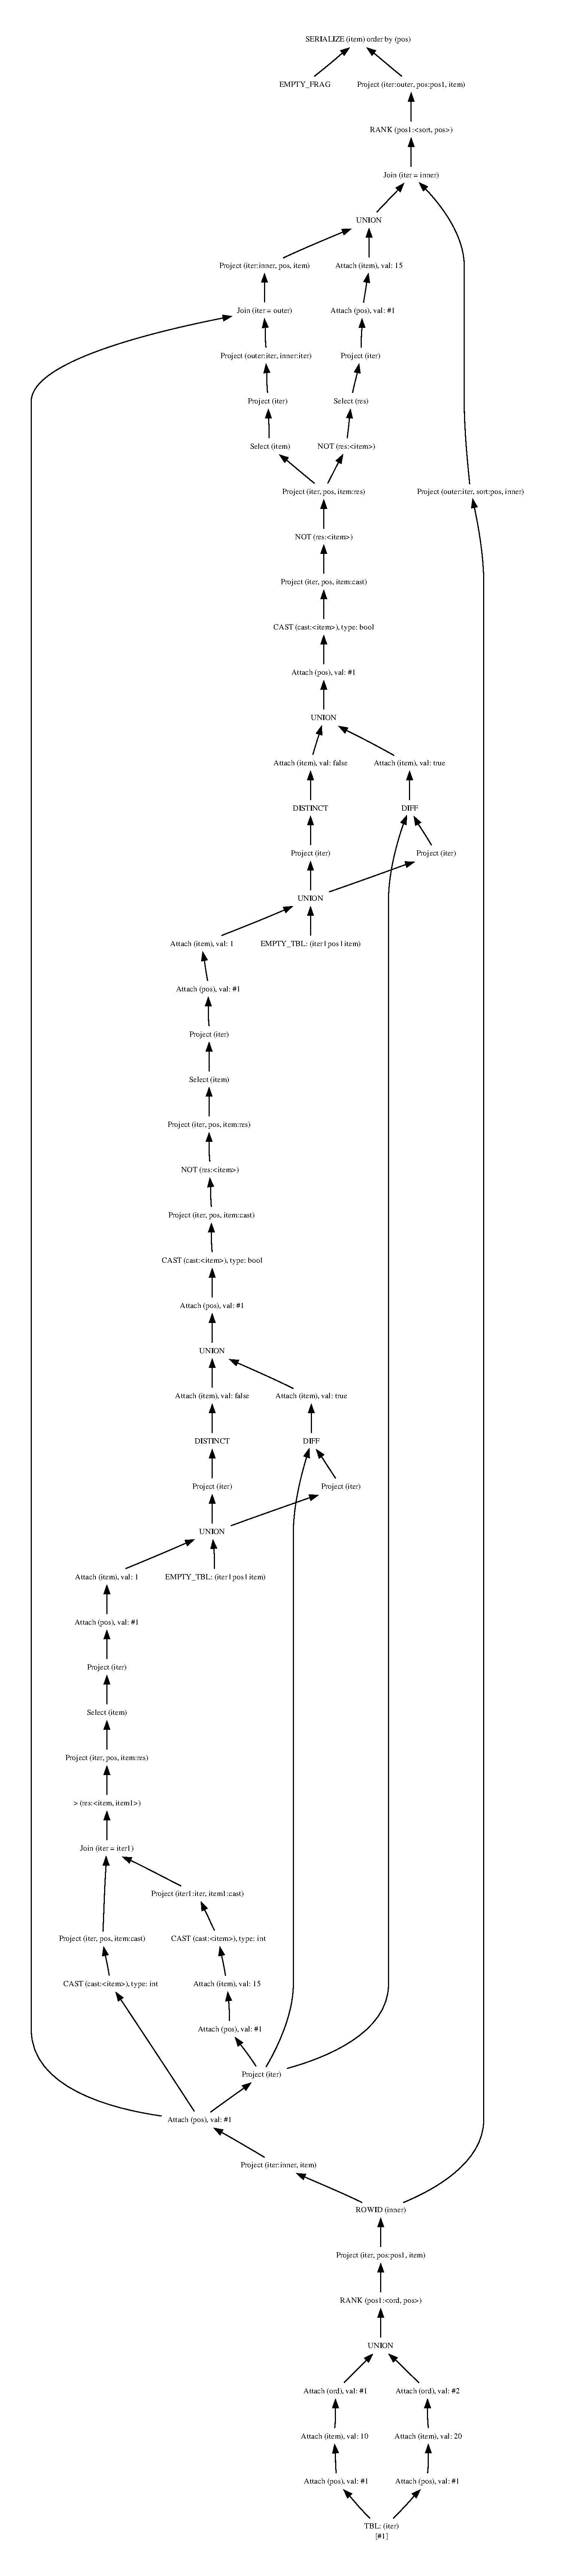
\includegraphics[width=0.3\textwidth]{img/graphs/td_impl_flwor_ifthenelse_pathfinder}
			\label{fig:result:comparison:conditional_dag}
		}
		\quad
		\subfigure[Prototype implementation]{
		
			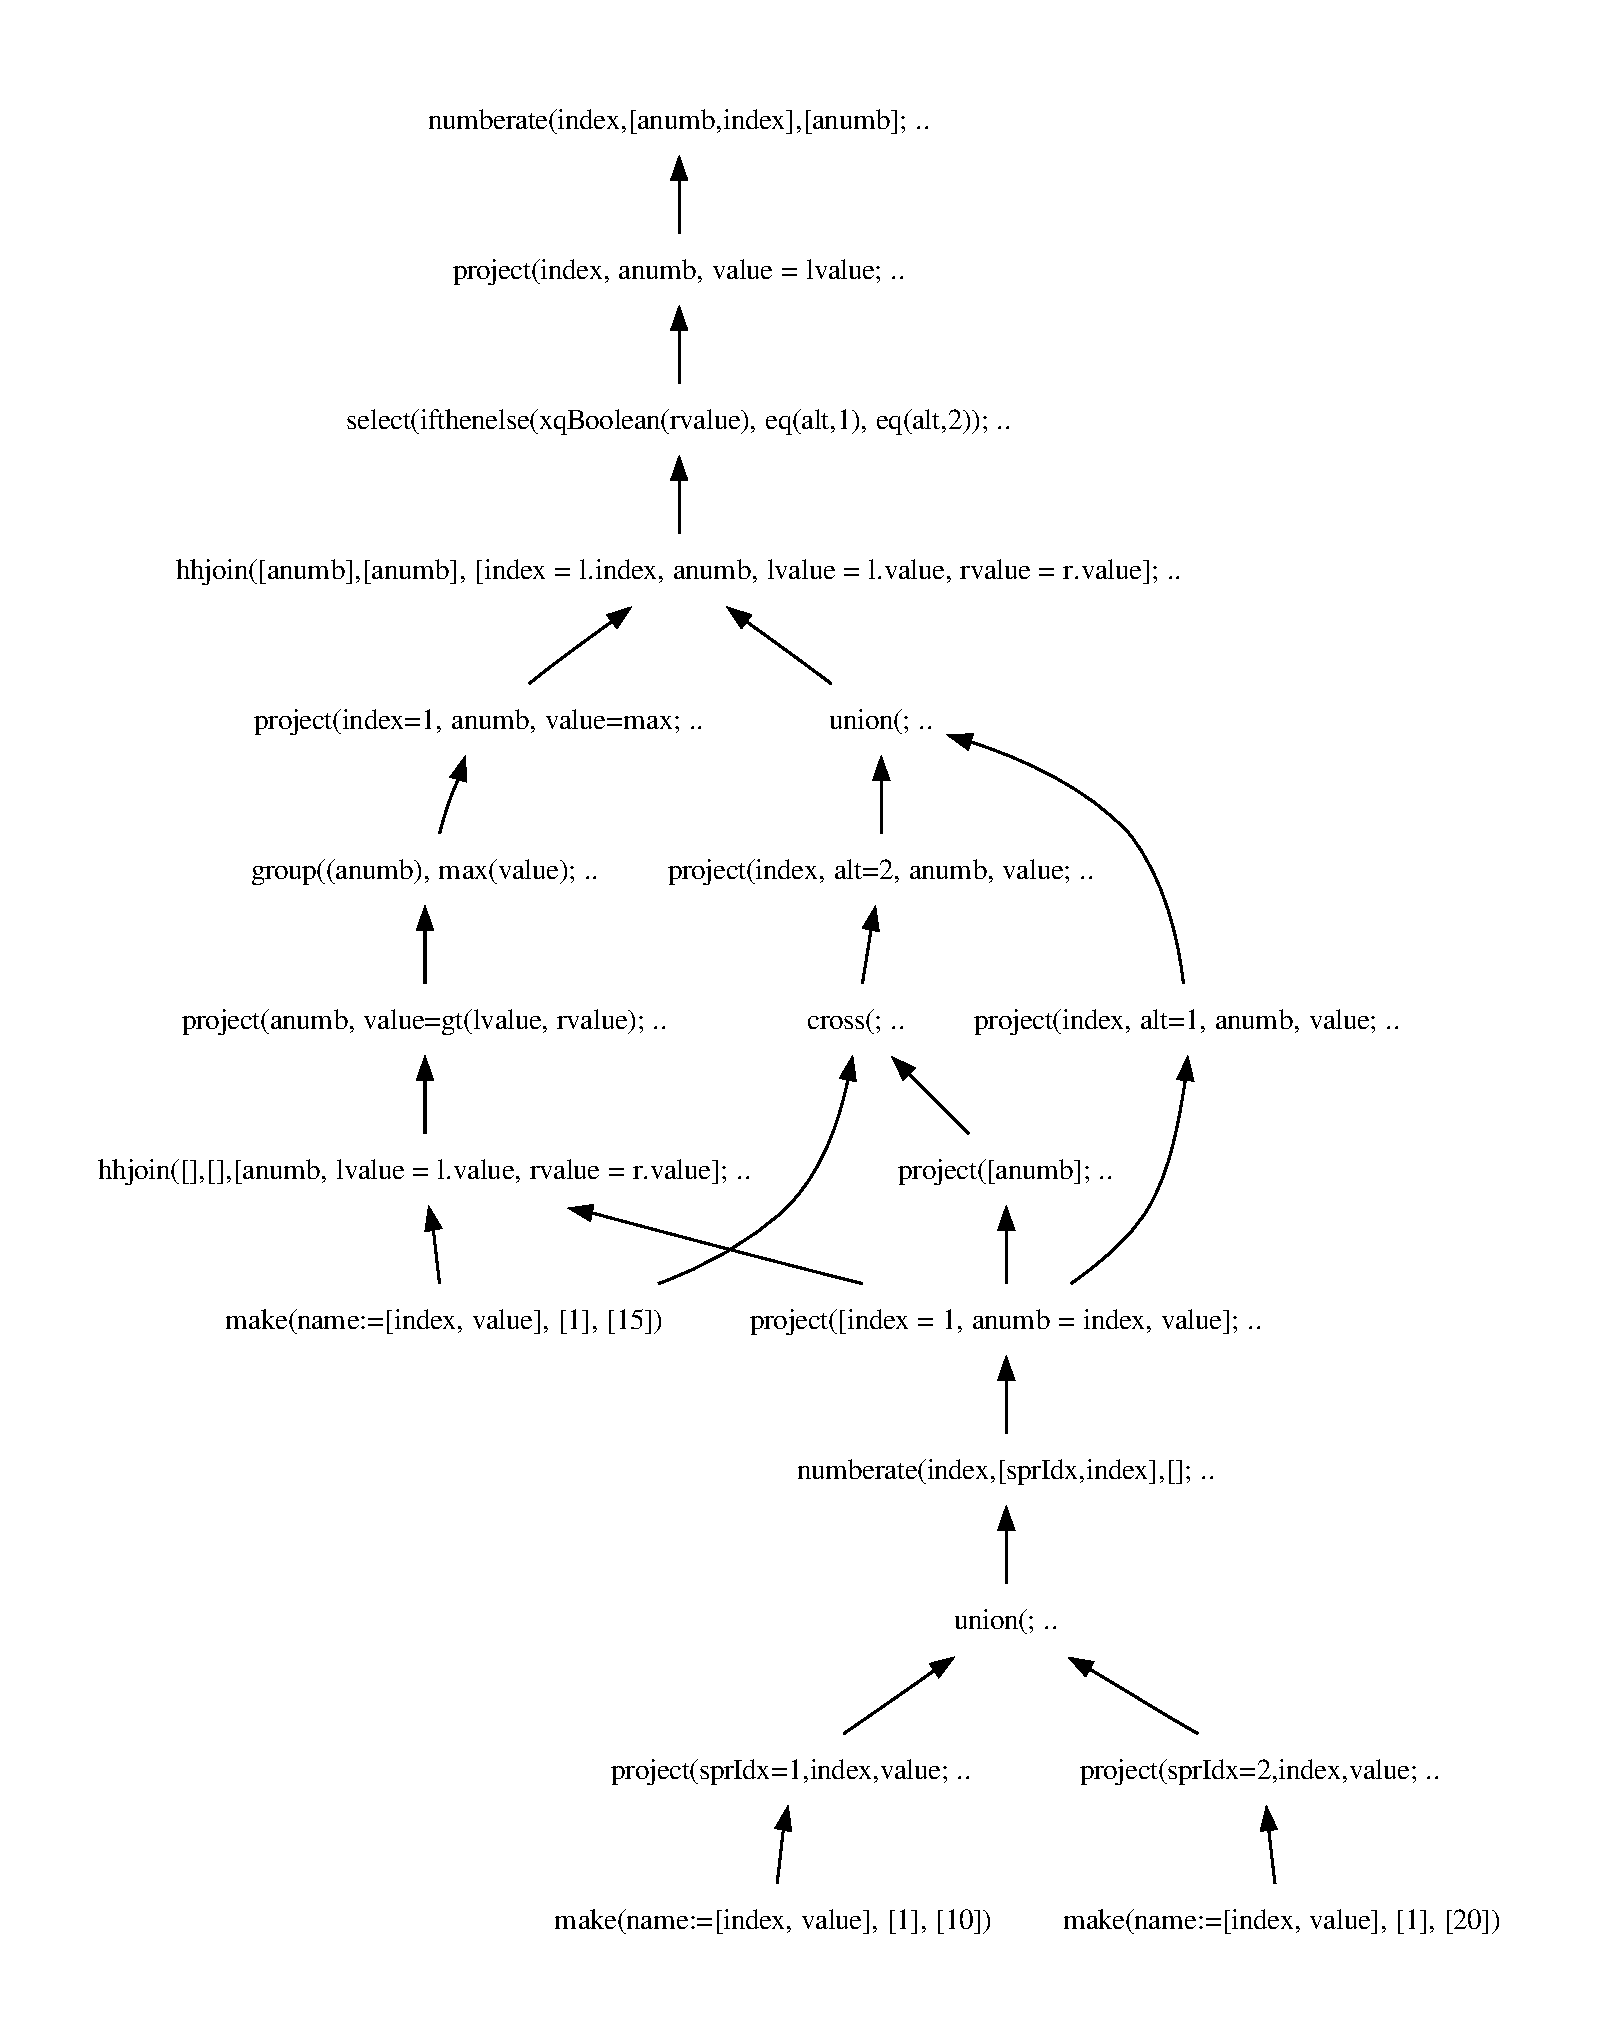
\includegraphics[width=0.7\textwidth]{img/graphs/td_impl_flwor_ifthenelse_xq_relalg_dag}
			\label{fig:result:comparison:conditional_pathfinder_dag}
		}
	}
	\caption{Comparison of DAGs for the conditional expression in section
	\ref{sect:results:algebra:generated:conditional_flwor}}
\end{figure}

\newpage
\begin{figure}[!h]
	\centering
	\mbox{
		\subfigure[Pathfinder/MonetDB]{		
			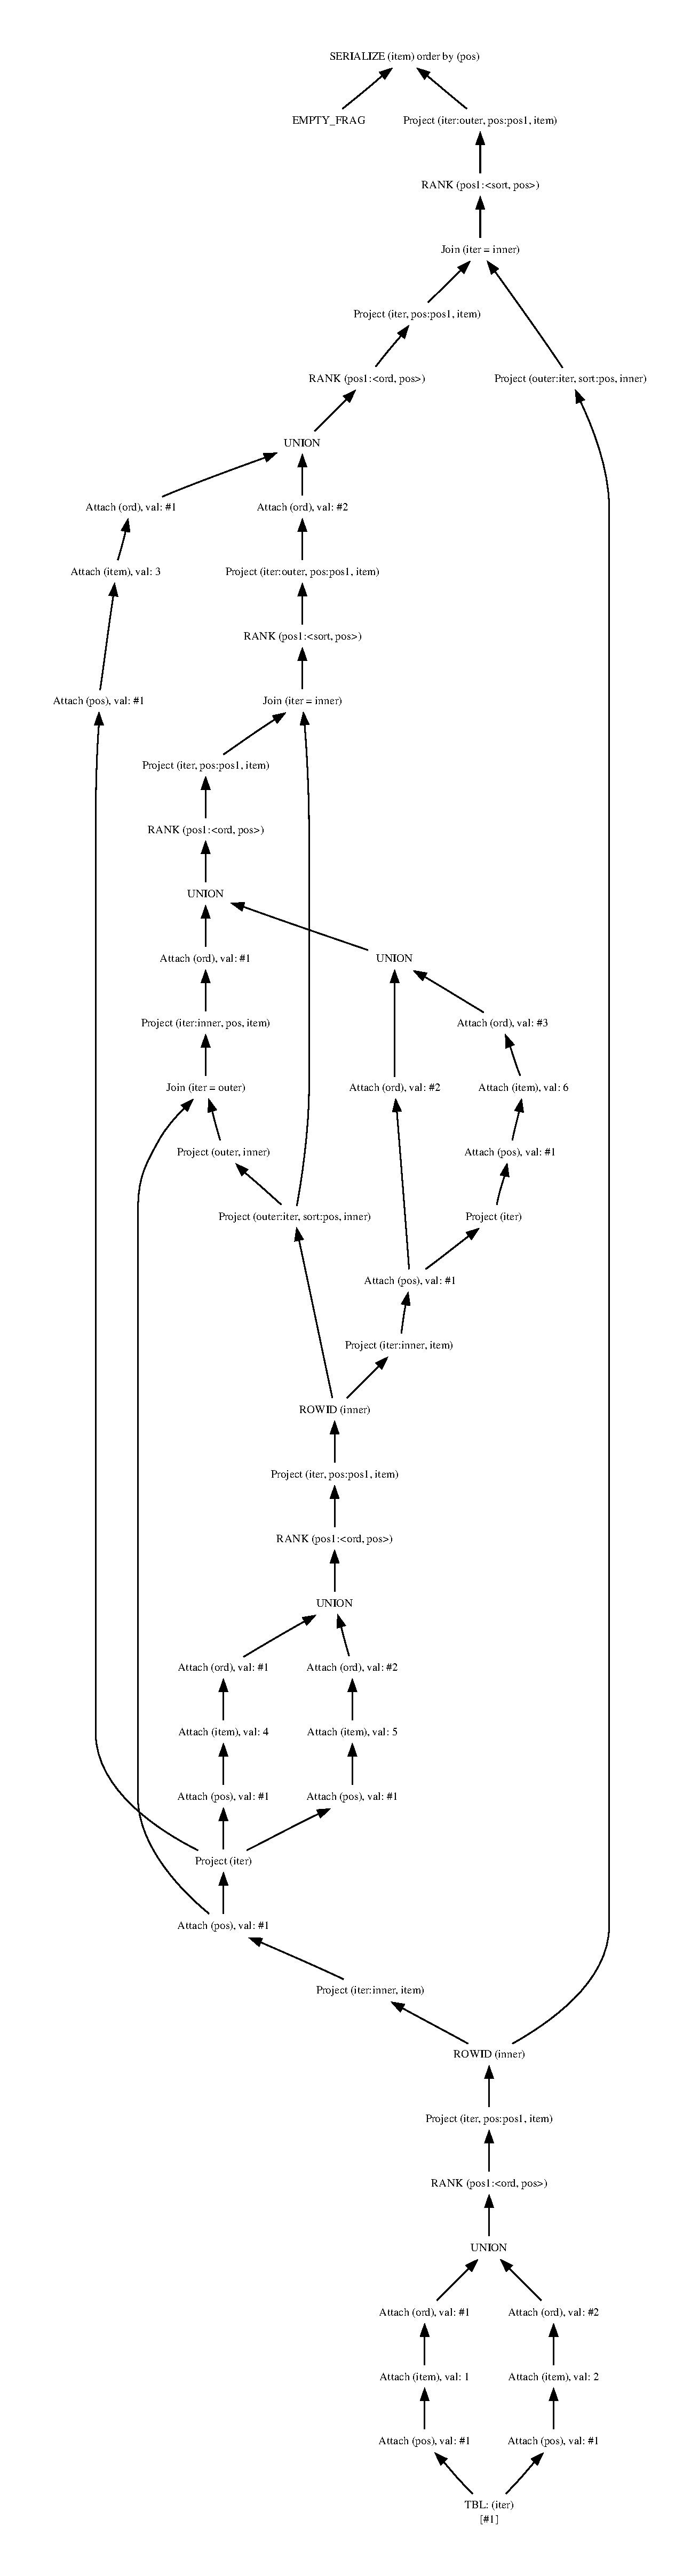
\includegraphics[width=0.37\textwidth]{img/graphs/td_impl_flwor_complex_pathfinder}
			\label{fig:result:comparison:complex_xqft_dag}
		}
		\quad
		\subfigure[Prototype implementation]{
		
			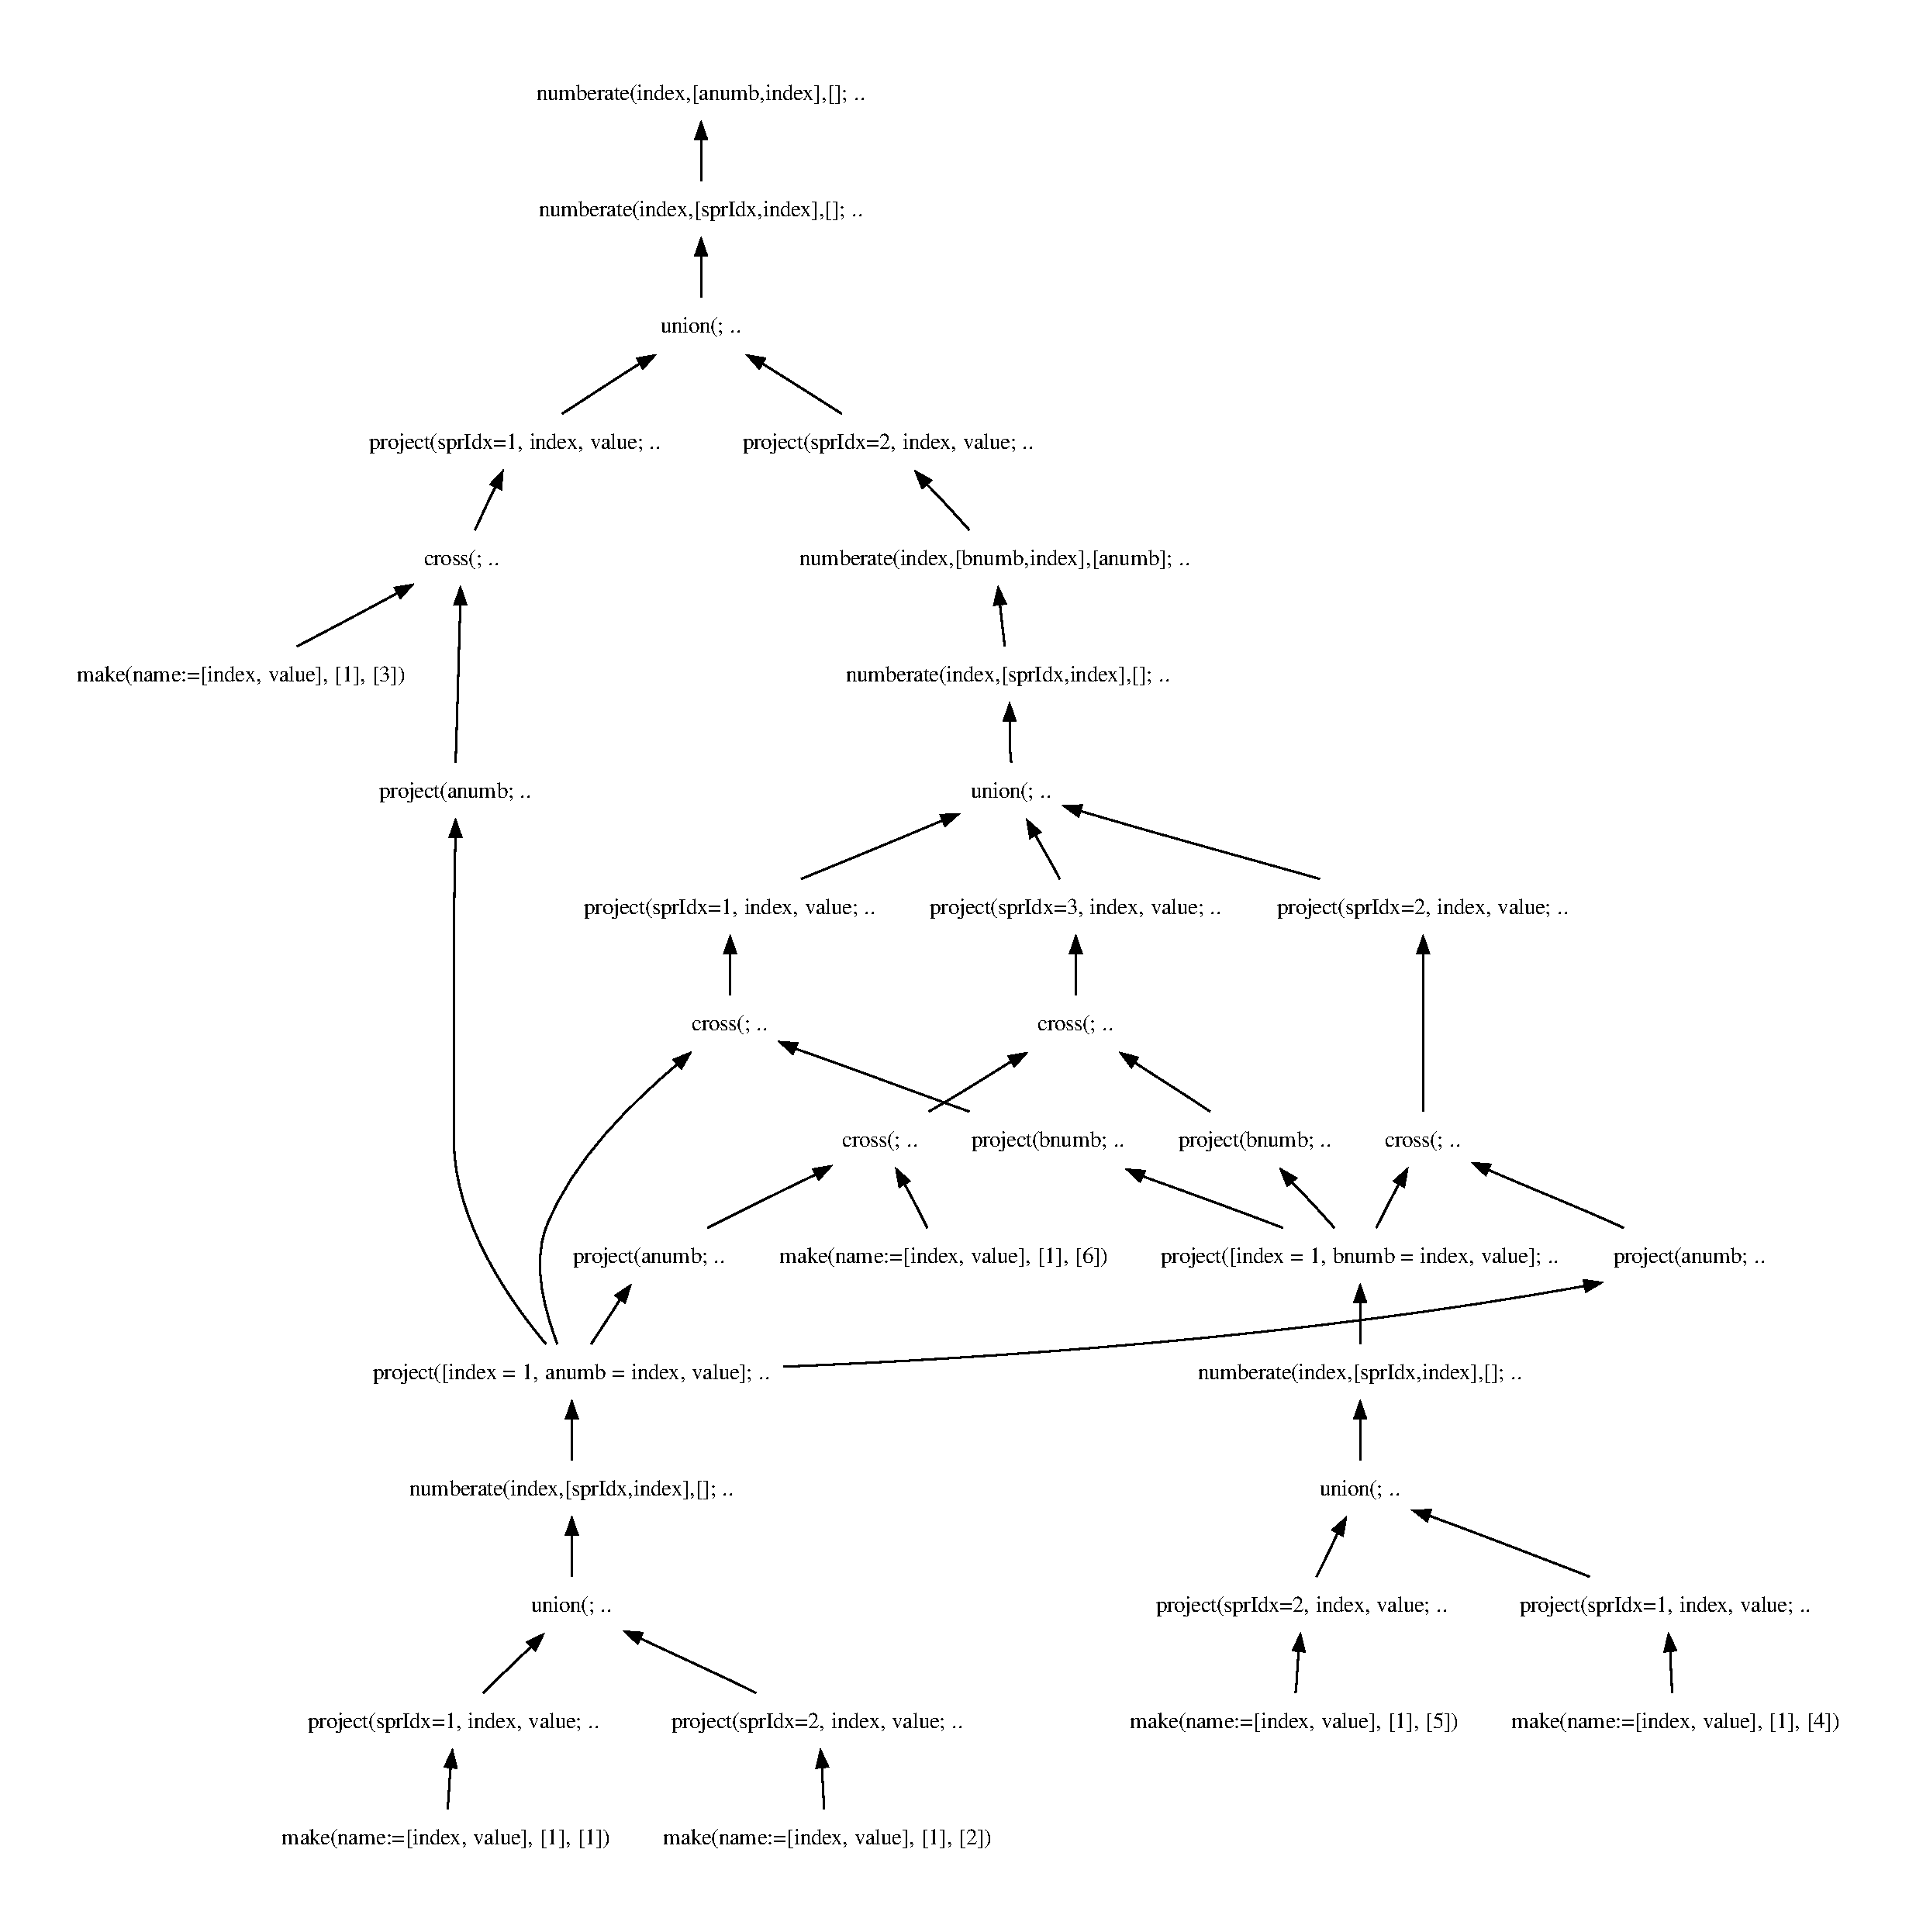
\includegraphics[width=0.6\textwidth]{img/graphs/td_impl_flwor_complex_xq_relalg_dag}
			\label{fig:result:comparison:complex_pathfinder_dag}
		}
	}
	\caption{Comparison of DAGs for the complex expression in section
	\ref{sect:results:algebra:generated:complex_flwor}}
\end{figure}

\newpage
\subsection{Complexity estimation and comparison}
Complexity estimation is performed as detailed in section
\ref{sect:method:complexity}. The complexity
comparison matrix is shown in table \ref{table:result:complexity_matrix}.

\begin{table}[!htp]
 \begin{tabular}{| c | c | c || c | c |}
  \hline
   & \multicolumn{2}{|c||}{\textbf{Pathfinder/MonetDB}}
   & \multicolumn{2}{|c|}{\textbf{Prototype implementation}} \\
   \hline
   & Tuples & Fields & Tuples & Fields \\  
   \hline
   Trivial & 16 & 16 & 15 & 18 \\  
   \hline
   Complex & 215 & 265 & 136 & 102 \\
   \hline
   Conditional & 94 & 50 & 31 & 44 \\  
   \hline
 \end{tabular}
\caption{Complexity comparison matrix}
\label{table:result:complexity_matrix}
\end{table}

\begin{figure}[!htp]
\begin{center}
  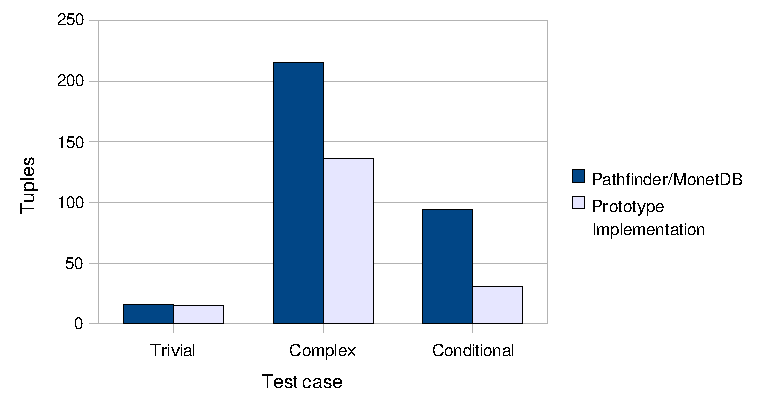
\includegraphics[width=1.0\textwidth]{diagrams/comparison_chart2_chart1}
  \caption{Comparison of complexity based on tuple creation}
  \label{fig:results:comparison:chart1}
\end{center}
\end{figure}

\begin{figure}[!htp]
\begin{center}
  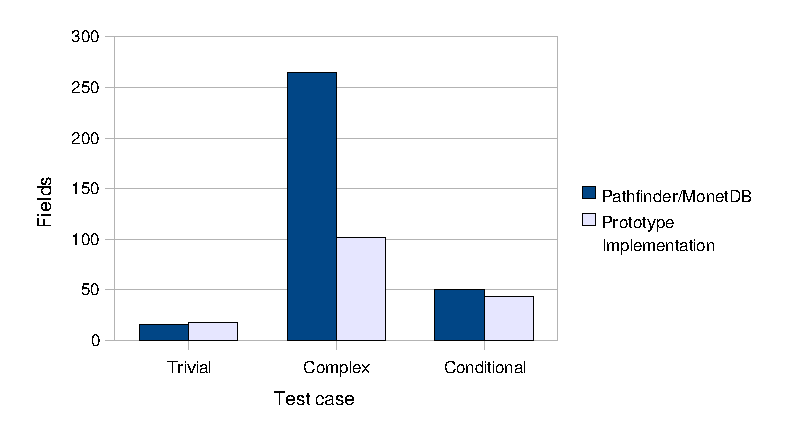
\includegraphics[width=1.0\textwidth]{diagrams/comparison_chart2_chart2}
  \caption{Comparison of complexity based on field creation}
  \label{fig:results:comparison:chart2}
\end{center}
\end{figure}
